%%This is the KMD un-official thesis template (Engineering Format for English Writer).
%
\documentclass[12pt,a4paper]{report}  % Should work with either pLaTeX or XeLaTeX
\usepackage{style/new-emthesis}
%
%%%%%%%%%%%%%%%%%%%%%%%%%%%%
%
% Decide what graphicx driver to use for images.
% For pLaTeX should use 'dvipdfmx'; default is OK otherwise.
\newcommand\gfxdriver{}
\ifXeTeX                        %% If XeLaTeX is being used
    \usepackage{fontspec}
    % Use standard TeX ligature logic
    \defaultfontfeatures{Ligatures=TeX}
    % Enable use of XeTeX CJK fonts for Japanese text if needed
    \usepackage[indentfirst=false]{xeCJK}
    % XeLaTeX also requires specifying CJK fonts
    %   (these must be TTF/OTF fonts installed on the computer)
    \setCJKmainfont{IPAMincho}      % Japanese serif (Mincho) font - e.g. MS PMincho
    \setCJKsansfont{IPAPGothic}     % Japanese sans (Gothic) font - e.g. MS PGothic
    \setCJKmonofont{IPAGothic}      % Japanese monospaced font - e.g. MS Gothic

\else\ifptex                    %% If pLaTeX is being used
    % Uncomment next 2 lines to enable ruby characters (furigana) if needed
    %\usepackage{pxrubrica}
    %\rubysetup{g}

    \renewcommand\gfxdriver{dvipdfmx}
\fi\fi
\usepackage[\gfxdriver]{graphicx}
%
%%%%%%%% Load other packages
\usepackage{parskip}
\usepackage{multicol}
\usepackage{mathrsfs}
\usepackage{amsmath}
\usepackage{listings}
\usepackage{color}
\usepackage{siunitx}
\usepackage{subcaption}
\usepackage{tabularx}
\usepackage{longtable}
\usepackage{multirow}
\usepackage{fancybox}
\usepackage{amssymb}
\usepackage{moreverb}
\usepackage{afterpage}
\usepackage{cite}
%\usepackage{harvard-oikos}
\usepackage{style/ccaption}           % caption
\usepackage{style/fn2end}             % footnotes script
\usepackage{style/fn2end_config}      % footnotes edit script
\usepackage{tabu}               % more powerful/flexible tables
\usepackage{fancyhdr}           % used to enable nice page headers
\ifptex
    \usepackage[hyphens]{url}           % format URLs nicely
\else                                   % also create links in document
    \usepackage[hidelinks,hypertexnames=false,hyperfootnotes=false]{hyperref}
    % Uncomment to enable ruby characters (furigana) if needed
    %\ifXeTeX \usepackage[CJK,nooverlap]{ruby} \fi
\fi

\lstset{frame=tb,
  aboveskip=3mm,
  belowskip=3mm,
  showstringspaces=false,
  columns=flexible,
  basicstyle={\small\ttfamily},
  numbers=none,
  numberstyle=\tiny\color{gray},
  keywordstyle=\color{blue},
  commentstyle=\color{dkgreen},
  stringstyle=\color{mauve},
  breaklines=true,
  breakatwhitespace=true,
  tabsize=3
}

%
%%%%%%%%%% Other tweaks
\makeatletter
%
% Remove the number from subsection headings
%\renewcommand*{\l@subsection}{\@dottedtocline{2}{3.8em}{1.2em}}
%\renewcommand{\thesubsection}{\hskip-1.0em}
%
% Make in-page footnotes use regular numbers instead of superscripts (per CMS)
\renewcommand{\@makefntext}[1]{%
    \noindent
	\leftskip=1.5em
	\hskip-1.5em
	\makebox[1.5em][l]{\@thefnmark}{#1}
}
\setlength{\skip\footins}{\baselineskip}
\setlength{\footnotesep}{1.3em}
%
% Also use a tighter line spacing for endnotes
\let\saved@theendnotes\theendnotes
\renewcommand{\theendnotes}{%
    \setlength{\baselineskip}{1.3em}
	\saved@theendnotes
}
%
% Uncomment the following to include the abstract in the table of contents:
%\let\saved@eabstractpage\eabstractpage
%\renewcommand{\eabstractpage}{%
%    \addcontentsline{toc}{chapter}{\abstractname}
%    \saved@eabstractpage
%}
\makeatother
%%%%%%%%%%%%%%%%%%%%%%%%%%%%

%
%%%%%%%%%%
% Page Style Settings - Choose One
\pagestyle{final}               % Final Draft
%\pagestyle{draft}               % Drafts


%%%%%%%%%%%%%%%%%%%%%% Optional Styling Tweaks %%%%%%%%%%%%%%%%%%%%%%
%
% Uncomment one of these to change the default Latin font:
%\renewcommand*\rmdefault{bch}   % Charter
%\renewcommand*\rmdefault{pnc}   % Century Schoolbook

%
% Uncomment to adjust the default line spacing.  The defaults are 1.1 for
% English and 1.2 for Japanese.  For tighter spacing, 1.0 can be used.
%\renewcommand{\baselinestretch}{1.0}

%
% Add a nice header to each non-initial page (optional):
%
\pagestyle{fancy}
\setlength{\headheight}{13.6pt}
\renewcommand{\chaptermark}[1]{\markboth{\MakeUppercase{#1}}{}}
\renewcommand{\sectionmark}[1]{\markright{\thesection\hspace{1em}#1}}
\fancyhead{}
\makeatletter\if@twoside              % Two-sided (book) style layout
    \fancyhead[LE]{\footnotesize\leftmark}   % Chapter name on left-hand page
    \fancyhead[RO]{\footnotesize\rightmark}  % Section name on right-hand page
\else                                 % Regular (single-page) layout
    \fancyhead[L]{\footnotesize\leftmark}    % Chapter name at left side
    \fancyhead[R]{\footnotesize\rightmark}   % Section name at right side
\fi\makeatother

%
% Table padding for use with tabu (only if \usepackage{tabu} specified above)
\setlength{\tabulinesep}{3pt}   % Vertical padding between rows

%
% Adjust space around float captions
\setlength{\abovecaptionskip}{0.5em}    % Space above bottom captions
\setlength{\belowcaptionskip}{1em}      % Space below top captions
\setlength{\parskip}{1em}

%
%%%%%%%%%%%%%% Thesis Parameters - Edit as Appropriate %%%%%%%%%%%%%%
%
%
% Language Settings
%\lang{Japanese} % Japanese
\lang{English} % English

%
% Student ID number
\studentnumber{81923362}

%
% Choosing Masters Thesis or Report
\doctitle{\mastersthesis}       % Masters Thesis
%\doctitle{\mastersreport}      % Report
\graduateschool{Graduate School of Science and Technology}
\school{School of Integrated Design Engineering}
%
% What Degree to obtain
\major{\mediadesign}    % Degree of Media Design

% \graduateschool{}
%
% Title (in LaTeX)
\etitle{Numerical investigation on electrical and thermal characteristics in organic semiconductor films from the aspect of variable range hopping}
%
% Title (in plain text)
%   No need to set if the same as  (in LaTeX)
\eptitle{}

%
%Author's Name (in LaTeX)
\eauthor{Descouens Nicolas}
%
% Author's Name (in plain text)
%   No need to set if the same as in (in LaTeX)
\epauthor{}
\advisor{Professor Noda Kei}
%
% Academic Year
\syear{2021}
%\heiseiyear{24}            % only required for Japanese thesis
%\smonth{2}
%\sday{7}

%
% Advisors
%
%\echmembers{Professor Hideki Sunahara}{(Supervisor)}
%          {Professor Akira Kato}{(Co-supervisor)}
%
% Thesis committee members - Supervisor, Co-supervisor, and Member must be
% specified.  Uncomment and edit ONE of these depending on the total number:
%
% If 5 advisors:
% Supervisor, Co-supervisor, and Member must be specified.
%\ecomembers{Professor Shunsuke Uemura}{(Supervisor)}
%          {Professor Minoru Ito}{(Co-supervisor)}
%          {Associate Professor Masatoshi Yoshikawa}{(Member, Nagoya University)}
%          {Associate Professor xxxxxx xxxxxx}{(Member)}
%\eaddcomembers{Associate Professor oooooo oooooo}{(Member)}
%
% If 4 advisors:
%\ecomembers{Professor Hideki Sunahara}{(Supervisor)}
%          {Professor Akira Kato}{(Co-supervisor)}
%          {Professor Nobuo Kawaguchi}{(Member, Nagoya University)}
%          {Associate Professor xxxxxx xxxxxx}{(Member)}
%
% If 3 advisors:
% \advisor{Hideki Sunahara}
% If 2 advisors:
% \ecomembers{Professor Hideki Sunahara}{(Supervisor)}
%           {Professor Akira Kato}{(Co-supervisor)}
%
% 5 or 6 Keywords (in LaTeX)
%
\ekeywords{}
%
% 5 or 6 Keywords (in plain text)
%   No need to set if the same as in (in LaTeX)
%\epkeywords{Design Thinking, Creative Society, Workshop, Innovation, Education}

%
%Choose one submission category from [Design, Science / Engineering, Social Science / Humanities, Action Research]
\ecategory{Science / Engineering}
%Choose one submission category from [Design, Science / Engineering, Social Science / Humanities, Action Research] (in plain text)
\pecategory{Science / Engineering}


%%%%%%%%%%%%%%%%%%%%%%%%%%Abstract%%%%%%%%%%%%%%%%%%%%%%%%%%%%%%%%%
\eabstract{The localization of states in organic semiconductor have caused some troubles at providing a viable thermal and electric transport. Understanding better the process in organic semiconducor could help improve the performances of many devices. We propose in this thesis to study the Einstein relationship and thermal conduction in regard of doped semiconductors which could be usefull for both understanding carrier transport and heat transport and also to engineer more efficient devices.

From the standpoint of the Variable Range Hopping (VRH) theory, we will compute models for both electric conduction and diffusion for classic organic semiconductors to finally be able to assess the Einstein ratio. We will perform simulation to grasp the influence of some parameters: doping, field, carrier density, energetic disorder, Fermi level. The model predicts value in accordance with the precedent litterature for most que the quantities, excepted the temperature and the Fermi level. To confirm our electric model, we used pentacene hole-only data measured by a precedent student and have found the numerical values for reasonable field to be in range with what was measured.

The background developped for the electric conduction has also been used to predict thermal conduction values for both phonons and charge carriers. Our approximated model succeeded in obtaining reasonable values in range with the litterature.

A special attention has been dedicated into developping a performing model in Julia and improving the performances without harming the precision and accuracy of the model.
}
%%%%%%%%%%%%%%%%%%%%%%%%% document starts here %%%%%%%%%%%%%%%%%%%%%%%%%%%%

%%%% No need to edit these

\begin{document}
%
%
\titlepage
\comemberspage
\firstabstract
%\secondabstract            % only required for Japanese thesis


%
%%%%%%%%%%%%%%%%%%%%%%%% Acknowledgements here %%%%%%%%%%%%%%%%%%%%%%%
\acknowledgements


%
%%%%%%%%%%%%%%%%%%%%%%%%%%%% Main Matter %%%%%%%%%%%%%%%%%%%%%%%%%%%%%
%
%Table of Contents and related matter
\toc
\newpage
\listoffigures
%
\newpage
\pagenumbering{arabic}

%
%%%%%%%% Chapters - input individual chapters here
%
% !TeX root = document-en.tex

\chapter{Introduction}
\label{chap:intro}

\makeendnotes  %make notes at the last of this chapter // if you do not  want use endnotes style, please comment out this.

\section{Organic semiconductors}

\subsection{Background}

For the past century, inorganic materials have been at the heart of the semiconductor industry, with element such as silicon, germanium or gallium arsenide. But, the industry turned itself to new devices and organics semiconductor are one of them. Their different set of properties: very flexible, low cost, less polluting helped them to gain interest.

More specifically, in 1977, the first highly conducting polymer was found, chemically doped polyacetylene, was discovered \cite{polyacetylene}. Such materials can be easily processed by techniques already know in the industry: vacuum evaporation, solution casting\dots But a better understanding and control of the self-assembly of molecules, as well as a booming research field, have increased greatly the performances, reaching the charge carrier mobility of amorphous silicon for some of them (fig. \ref{fig:1}). The high diversity of geometry within the material allows a better tuning of the characteristic of the semiconductor to the use. One greater advance is the combination of both organic and inorganic molecules, particularly with perovskite. The high mobility of inorganic material combined with the more flexible geometry of organic ones make possible the creation of devices that reaches the performances of single-crystal silicon \cite{IBM,perovskite}.

\begin{figure}
    \centering
    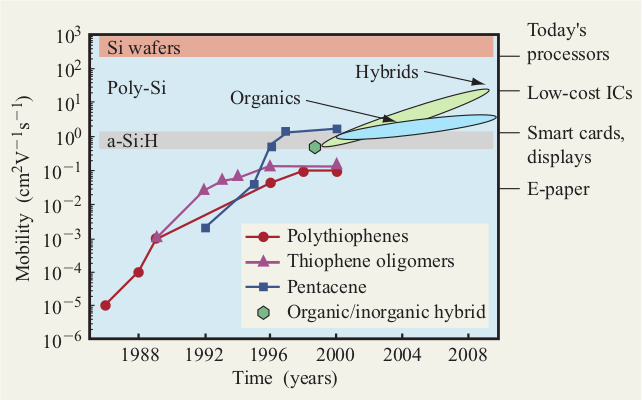
\includegraphics[width=.6\paperwidth]{figures/evolution_perf.png}
    \caption{Evolution of the performance for some organic semiconductors \label{fig:1}\cite{IBM}}
\end{figure}

This new development has been seen through the recent appearance of organic devices in the market. The more flagrant one is OLED devices, they offer a better diversity (flexible screens) with increased performance (higher color fidelity, darker black and better contrast) as well as consumption. But it's also used in professional devices such as OTFT \cite{OTFT}, laser diode \cite{laserDiode}, \dots

\subsection{Organic materials}

Organic molecule are bound to each other by $\pi - \pi$ bounding which are the result of $p_z$-orbitals of $sp^2$-hybridized C-atoms in the molecules (fig. \ref{fig:2}). Such bonding is way weaker compared to the classic $\sigma$-bounding in the molecule backbone. Therefore, the $\pi-\pi^*$ transitions have a typical lower gap: around $\SI{1.5}{eV}-\SI{3}{eV}$ (fig. \ref{fig:3}). Their crystallinity ranges from single-crystal (pentacene, rubrene crystals) \cite{mono_crystal} to completely amorphous semiconductors like $\alpha$-NPD \cite{amorphous}.

\begin{figure}
    \centering
    \includegraphics*[width=0.4\paperwidth]{figures/pi_bonding.png}
    \caption{$\sigma$ and $\pi$ bonds in ethene \label{fig:2} \cite{intro_orga}}
\end{figure}

\begin{figure}
    \centering
    \includegraphics*[width=0.4\paperwidth]{figures/pi_pistar.png}
    \caption{$\pi-\pi^*$ bonding \label{fig:3} \cite{intro_orga}}
\end{figure}

Those weaker Van der Waals bonding lead to more localized charge carrier in the material. Most of the time, charge carriers do not evolve in bands like in Si, but are subject to a HOMO (Highest Occupied Molecular Orbital) and LUMO (Lowest Unoccupied Molecular Orbital) states. It results in a much weaker wavefunction delocalization for the neighboring molecules \cite{intro_orga}. Instead of band transport, organic materials are subject to hopping transport: a charge carrier hop from a site to an other and thus participate to the general conduction (fig.\ref{fig:4}). The difference between trapping and hopping state is in the recombination and release rate. if the former one is higher than the letter one, the state is a recombination center, otherwise, it is a trap. In this model the difference between trapping states and recombination states can be thin.

\begin{figure}
    \centering
    \includegraphics*[width=0.4\paperwidth]{figures/hopping_theory.png}
    \caption{Hopping transport \label{fig:4}}
\end{figure}

Organic semiconductors are divided between polymers and small molecules. The separation occurs at $1000$ molecular weights. Small molecules can achieve high cristallinty but are less soluble in solvent, requiring dry processes such as vacuum deposit, which is more difficult and more costly. On the other hand, polymer are easier to made in organic solvents. Even though small molecules show better performances, they're less stable than polymer in atmospheric conditions.

\subsection{Charge carrier transport}

As it has been said before, disorganized organic semiconductors are the place of localized charge carrier transport, and in the 70's, a theory has been proposed involving tunneling between near states \cite{hopping_theory_1}. Such theory as been previously discovered by Mott based on the dependence of the mobility on the temperature: an increasing temperature leads to an increasing mobility. This relation has been verified in practical devices \cite{hopping_theory_1,multiple_theory}.

In the variable range hopping theory (VRH), the displacement between two states for a charge carrier is determined only by the difference in energy $W$ and in position $R$, thus highlighting the fact that our system is resolutely in 4D. On top of that, we assume that the system is so disordered that this two quantities are decoupled. The jump frequency is usually described by the Miller-Abrahams formalism \cite{miller}:

\begin{equation}
    \nu=\nu_{0}\left\{\begin{array}{r}
    \exp \left(-2 \alpha R_{i j}-\frac{E_{j}-E_{i}}{k_{B} T}\right): E_{j}-E_{i} \geq 0 \\
    \exp \left(-2 \alpha R_{i j}\right): E_{j}-E_{i} \leq 0
    \end{array}\right.
    \label{eq:1}
\end{equation}

\begin{itemize}
    \setlength\itemsep{0.1em}
    \item $\nu_0$: base-jump frequency
    \item $R_{i j}$: distance between initial state $i$ and final state $j$
    \item $\alpha$: decay constant of the assumed hydrogen-like localized state wave functions
    \item $E_i$: energy of the state $i$
\end{itemize}

Depending on the position of the final state $j$, the formula change. If the state is on higher energy, it requires tunneling to occur on the energetic part, whereas if the reaching state if of a lower energy, only the distance is taken into account for the tunneling effect.

Using this formalism, it is possible to access the mobility and diffusivity for charge carrier.

\subsection{The einstein relation}

\subsubsection{Classical einstein relation}

\begin{equation}
    \frac{D}{\mu} = \frac{k_bT}{q}
    \label{eq:2}
\end{equation}

\begin{itemize}
    \setlength\itemsep{0.0em}
    \item $\mu$: mobility
    \item $D$: diffusion
    \item $k_B$: Boltzmann constant
    \item $T$: temperature
    \item $q$: elementary charge
\end{itemize}

The einstein relation \cite{einstein}, is a useful equation that link two quantities, $\mu$ and $D$ over a simple equation. $D$ constitutes a key parameter in analyzing semiconductor but is not so easy to measure. On the contrary, the mobility is easily accessed. However, in the presence of energetic disorder, such simple equation does not seem to hold \cite{ein_drift,ein_drift_2}. In non-equelibrium cases, it also seems that we can't use this relation anymore, the relation between the diffusion and the field seems to be quadratic \cite{diffusion_F}.

\subsubsection{Generalized equation}

From the limit of the eq. \ref{eq:2}, a new relation has been proposed, taking into account the dependence on the carrier concentration \cite{generalied_quasi}:

\begin{equation}
    \frac{D}{\mu}=\frac{n}{q \partial n / \partial E_{F}}
    \label{eq:3}
\end{equation}

\begin{itemize}
    \setlength\itemsep{0.0em}
    \item $E_F$: quasi-Fermi level
    \item $n$: carrier concentration
\end{itemize}

With $n$ being the carrier concentration defined by the fermi-dirac distribution $f = \frac{1}{1 + exp\left(\frac{E - E_F}{k_BT}\right)}$ and $g$ the gaussian density of state \cite{generalied_quasi}:

\begin{equation}
    n=\int_{-\infty}^{\infty} \frac{g(E)}{1+\exp \left(\frac{E-E_{F}}{k_{B} T}\right)} d E
    \label{eq:4}
\end{equation}

Such eq. \ref{eq:4} has been calculated following the hypothesis that drift and diffusion of charge carrier at fermi level are exactly compensated, meaning that there is no net current and is only valid for low electric field.

From this stating, a more suitable equation has been proposed in the following thesis.

\subsection{Gaussian density of states}

\begin{equation}
    g(E)=\frac{N}{\sigma \sqrt{2 \pi}} \exp \left(-\frac{E^{2}}{2 \sigma^{2}}\right)
    \label{eq:5}
\end{equation}

Gaussian density of states has been suggested by numerous monte-carlo simuations \cite{DOS_monte_carlo} as well by the observation of the excitonic absorption profile which is gaussian too. Besides, the intrinsic localization behavior of the gaussian density of state fit very well the observation made on real devices.

From a mathematical point of view, the disorder is directly linked to $\sigma$, which broadens the bell-shaped of the function (fig. \ref{fig:5}, \ref{fig:6}).

\begin{figure}
    \centering
    \includegraphics*[width=.5\paperwidth]{figures/DOS_1.png}
    \caption{Gaussian DOS, $\sigma=1$ \label{fig:5}}
\end{figure}

\begin{figure}
    \centering
    \includegraphics*[width=.5\paperwidth]{figures/DOS_3.png}
    \caption{Gaussian DOS, $\sigma=3$ \label{fig:6}}
\end{figure}

\subsection{Thermal diffusion}

Organic semiconductors have recently received much attention regarding their potential thermoelectric effect. From their figure of merit (eq. \ref{eq:6})

\begin{equation}
    \mathrm{ZT}=\frac{\sigma \cdot S^{2}}{\kappa} T
    \label{eq:6}
\end{equation}

\begin{itemize}
    \item $S$: Seebeck coefficient
    \item $\sigma$: electrical conductivity
    \item $\kappa$: thermal conductivity
\end{itemize}

From ZT value is representative of the electric efficiency of the device. Thus a lower thermal conductivity $\kappa$ naturally leads to higher figure of merit and to an increased energetic conversion.

A better understanding of the process is key to engineering better devices, but the classical theory used on inorganic material \cite{einstein_model_thermic} can't be applied directly to organic ones. The variety of morphology in organic semiconductors plays a great role in defining its thermal characteristics and is extremely sensitive to the spacial arrangement of the molecules within the material.

To simulate the thermal effect, one should take into account both charge carrier and phonon transport: $\kappa = \kappa_e + \kappa_p$ with a slight predominance of the phonon in the process of thermal conduction \cite{universal_einstein}.

\section{Objectives of this thesis}

The overall understanding of both electric and thermal behavior of organic semiconductors is scarce. Their great diversity, which is at the heart of their recent success, makes it difficult to get an simulation of the charge carrier in the material. The goal of this thesis is to obtain, thanks to equations developed throughout the 20th century and to new hypothesis on the comportment of the charge carrier, as well as a powerful computer language, a reasonable approximation of the electric and thermal figures in doped organic semiconductors. Our objectives are:

\begin{itemize}
    \item Estimate einstein ratio for many type of organic semiconductors
    \item Estimate the thermal conduction by taking into account both charge carrier and phonon participation
    \item Take into account the doping behavior of the semiconductor, as well as the disorder and electric effect
    \item Simulate the behavior in a fairly small amount of time
\end{itemize}

The novelty of this study resides in the multitude of the parameters taken into account and in new behavior for charge carrier within the material.

%%%%%Notes%%%%%
% if you do not  want use endnotes style, please comment out the below.
% \section*{Notes}
% \addcontentsline{toc}{section}{Notes}
% \begin{footnotesize}
% \theendnotes
% \end{footnotesize}
% !TeX root = document-en.tex

\chapter{Electric properties}
\label{chap:elec}

The framework for the electric properties, diffusion, mobility and einstein ratio will be detailed in this section. As now on, we will adopt the following formalism. If not stated otherwise, every quantity written in lowercase will be reduced and all the quantity in uppercase will be the non-reduced equivalent ($u_F$ is the reduced quantity of $U_F$). To reduce the unit we will use respectively for the energetic dimension and spatial dimension:

\begin{equation}
    \begin{aligned}
        u &= \frac{U}{k_bT}\\
        r &= 2\alpha R
    \end{aligned}
\end{equation}

$k_B$ being the Boltzmann constant and $\alpha = \SI{4.34e7}{cm^{-1}}$ the decay constant of the assumed hydrogen-like localized state wave functions.

\section{Gaussian formalism}

To simulate the localized behavior of charge carrier, we will use a gaussian density of states (gaussian DOS) for doped semiconductor. The doping effect will take form of an another gaussian with a different peak. The origin of the energy will be taken to be the LUMO level, but this theory works for holes and electron alike: an energy inversion is will bring us into the hole formalism.

\begin{equation}
    \begin{aligned}
    g\left(E, \hbar \omega_{\alpha}\right)=& \frac{1}{\sqrt{2 \pi}}\left\{\frac{N_{i-e}}{\sigma_{i}} \exp \left(-\frac{\left(E-\hbar \omega_{\alpha}\right)^{2}}{2 \sigma_{i}^{2}}\right)\right.\\
    &\left.+\frac{N_{d-e}}{\sigma_{d}} \exp \left(-\frac{\left(E-\hbar \omega_{\alpha}+E_{d}\right)^{2}}{2 \sigma_{d}^{2}}\right)\right\}
    \end{aligned}
    \label{eq:DOS_e}
\end{equation}

\begin{itemize}
    \item $N_{i-e}(cm^{-3})$: density of charge carriers for the intrinsic material
    \item $N_{d-e}(cm^{-3})$: density of charge carriers for the doped material
    \item $\hbar \omega_\alpha(J)$: mode effect, vibration of the lattice
    \item $\sigma_i(J)$: width of the intrinsic gaussian, representative of the disorder of the intrinsic material
    \item $\sigma_d(J)$: width of the doped gaussian, representative of the disorder of the doped material
    \item $E_D(J)$: energy shift between intrinsic and doped material
\end{itemize}

$g_e$ is expressed in $cm^{-3} J^{-1}$.

On the figure \ref{fig:3_2}, the doping results in a broadening of the DOS, which is coherent with doping increasing the number of states within the material.

\begin{figure}[htbp]
    \centering
    \begin{subfigure}[t]{0.49\textwidth}
        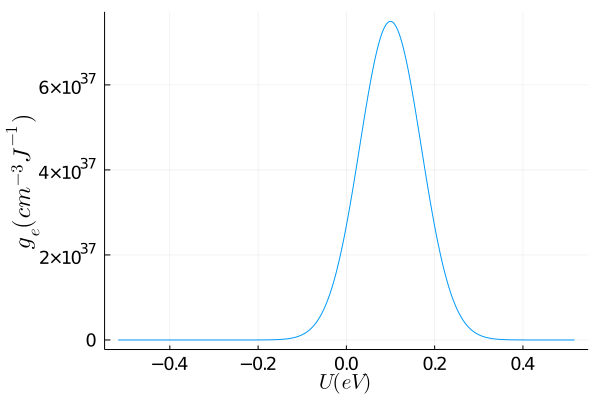
\includegraphics[width=\textwidth]{figures/3_elec/dos_undoped.png}
        \caption{Non-doped semiconductor}
    \end{subfigure}
    \begin{subfigure}[t]{0.49\textwidth}
        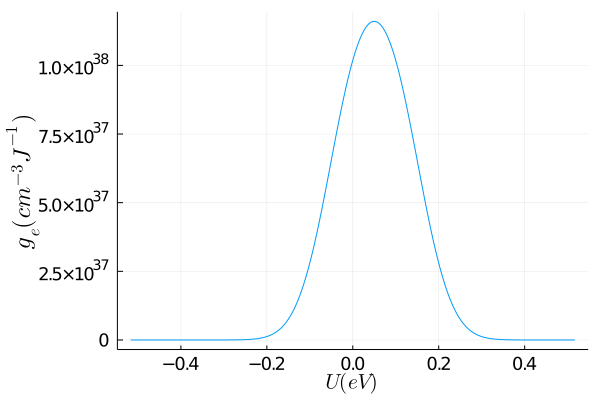
\includegraphics[width=\textwidth]{figures/3_elec/dos_doped.png}
        \caption{Doped semiconductor \\ $N_{d-e} = \SI{2.1e18}{cm^{-3}}$, $E_D = \SI{0.1}{eV}$}
    \end{subfigure}
    \caption[DOS]{DOS doping comparison \\ $T = 300K$, $N_{i-e} = \SI{2.1e18}{cm^{-3}}$, $\hbar \omega_\alpha = \SI{0.16e-19}{J}$}
    \label{fig:3_2}
\end{figure}

Using the Fermi-Dirac distribution, the carrier concentration is:

\begin{equation}
    n = \int_{-\infty}^{+\infty}\frac{g_e(U)}{1 + exp\left((\frac{U - (\hbar \omega_\alpha + U_F)}{k_BT}\right)}d U
\end{equation}

\section{Variable range hopping}

\subsection{Background}
We suppose that the charge carrier jump by tunneling from one state to another. The system is thus described in 4 dimensions: 3 for the spatial dimension, and one for the energy.

In our semi-classical model, we define the average probability for a jump to be the geometrical mean for all the jump within a material:

\begin{equation}
    \langle P \rangle = \operatorname{lim}_{n \rightarrow \infty}\left[\prod_{i}^{n} P_{i}\right]^{1 / n}=\exp \left[\operatorname{lim}_{n \rightarrow \infty} \frac{1}{n} \sum_{i}^{n} \ln P_{i}\right]
\end{equation}

$P_i$ being a singular jump in the material, we make the average over all the jump in the material.

As the arithmetic mean is more familiar, it's easier to work with the $\frac{1}{n} \sum_{i}^{n} \ln P_{i}$ part. To do so, we define the distance hopped to be:

\begin{equation}
    r_i = -ln(P_i)
\end{equation}

The $i$ arises from the fact that $P_i < 1$ and the logarithm is thus negative. Finally, we get:

\begin{equation}
    \langle P \rangle = exp(-r_{nn})
\end{equation}

With $r_{nn}$ being the mean range to the nearest neighbor for each state throughout the material. This theory making the average over all the states in the material has the advantage of summarizing the spatial and energy distribution of the states in on variable $r_{nn}$. The Miller-Abrahams hopping rate can now be written as:

\begin{equation}
    \nu = \nu_0 \cdot exp(-r_{nn})
    \label{eq:3_1.1}
\end{equation}

Usually, $\nu_0$ which is the basic hopping rate is set to $\SI{1e13}{Hz}$.

If we define $P_{ij}$ to be the probability of a jump from the state $i$ to the state $j$, from an energetic standpoint:

\begin{equation}
    P_{ij}^{energy} = exp\left(\frac{U_i - U_j}{k_BT}\right) = exp(u_i - u_j)
\end{equation}

From a spatial standpoint:

\begin{equation}
    P_{ij}^{spatial} = exp\left(-2\alpha L_{ij}\right) = exp(-l_{ij})
\end{equation}

We can fairly assume that:
\begin{equation}
    P_{ij} = P_{ij}^{total} = P_{ij}^{energy} \cdot P_{ij}^{spatial} = e^{[u_i - u_j] - l_{ij}} = e^{r_{ij}}
    \label{eq:3_1}
\end{equation}

We write the field effect as: $\beta = \frac{Fe}{2\alpha k_BT}$, $F$ being the field intensity in $V cm^{-1}$. Of course, the course of a charge carrier is modified by the field. To model this, we include it directly in the equation of the 4D distance: a state alongside the field direction will be seen as  closer or father depending on the angle $\theta$ between $R_{ij}$ and $F$:

\begin{equation}
    \left.\begin{array}{rlr}
    R_{i j} & =(1+\beta \cos \theta) L_{i j}+\left(U_{j}-U_{i}\right) & \text { for } U_{j}>U_{i}-\beta \cos \theta R_{i j} \\
    & =L_{i j} & \text { for } U_{j}<U_{i}-\beta \cos \theta R_{i j}
    \end{array}\right\}
    \label{eq:3_2}
\end{equation}

$(1+\beta \cos \theta)$ arises from the shift of the fermi level due to the field (fig. \ref{fig:R_max}). We assume here that for states to lower energy, only the physical distance is taken into account as the charge carrier does not need to make a jump to higher energies.

\subsection{Nearest neighbor}

The quantity $r_{nn}$ can be computed thanks to the formula of the "number of free states" $\mathscr{N}$, the mean number of free state at a distance $\mathscr{R}$ \footnote{Please note that the quantity $\mathscr{R}$ is reduced.} of a state. We suppose that the material is disorganized enough to make both energetic and spatial dimension uncorrelated, and that the states are equally distributed in respect of the gaussian DOS.

\begin{equation}
    \begin{aligned}
    \mathcal{N}\left(u, T, \beta, \mathscr{R}\right)=\int_{0}^{\pi} \int_{0}^{\mathscr{R}} \int_{-\infty}^{\mathscr{R}+u-r(1+\beta \cos \theta)} g\left(v\right)\left[1-F\left(v\right)\right] \frac{k_B T}{8 \alpha^{3}} \\
    \times 2 \pi r^2 \sin \theta d v d r d \theta
    \end{aligned}
    \label{eq:3_3}
\end{equation}

\begin{figure}[!h]
    \centering
    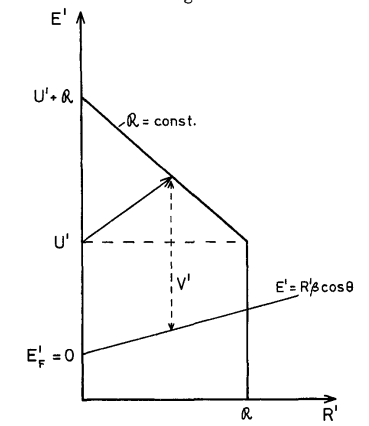
\includegraphics[width=.4\paperwidth]{figures/3_elec/R_max.png}
    \caption{Energetic-spatial relationship \label{fig:R_max} (source \cite{hopping_theory_1})}
\end{figure}

$g(1 - F)$ represent the emptiness of a state, $F$ being the Fermi-Dirac equation, $1 - F$ is the probability of the state to be empty, i.e a state where a charge carrier can jump. $\frac{k_B T}{8 \alpha^{3}}$ is simply a reducing factor to eliminate the unit of $g(1-F)$. $4\pi r^2$ is the surface of a sphere with a radius $r$ and $\frac{1}{2}\sin \theta$ makes the average between the field effect direction and the direction of $r$. The $\frac{1}{2}$ factor arises from the integral $\int_0^\pi \frac{1}{2}\sin \theta = 1$. The born in the energetic integral $\mathscr{R}+u-r(1+\beta \cos \theta)$ correspond to the maximum energetic value for a jump of distance $\mathscr{R}$. Finally, $\mathcal{N}$ computes the number of states enclosed enclosed in a 4D sphere of radius $\mathscr{R}$.

We thus define $r_{nn}$ being the radius at which we found in average, 1 free state, i.e $\mathcal{N}(r_{nn}) = 1$.

This method for computing $\mathscr{N}$ is similar to the percolation criteria, but they take $\mathcal{N}(r_{nn}) = 2.8$, $2.8$ being the percolation criteria. But, where the percolation theory intends to find a path of jump within the material, our $r_{nn}$ quantity means the nearest free states, which intuitively corresponds to the distance at which we find 1 state.

\begin{figure}[!h]
    \centering
    \includegraphics*[width=.5\paperwidth]{figures/3_elec/rnn.png}
    \caption{$r_{nn}$ behavior for pentacene, $F = \SI{5.3}{V . cm^{-1}}$ (pentacene parameters appendix \ref{pentacene})\label{fig:3_3}}
\end{figure}



From the figure \ref{fig:3_3}, we see that for low value of energy, the quantity $r_{nn}$ skyrockets. The rarefaction of available states due to the Fermi-Dirac distribution means that for a charge carrier to find an available spot is harder. On the opposite, we see a plateau at higher energetic values. At such energy, charge carrier can make energetically favorable jump to lower states, which depends only on the intrinsic characteristics of the material (the state distribution $g(1 - F)$). Mathematically, the born $\mathscr{R}+u-r(1+\beta \cos \theta)$ makes it happen: for lower $u$, $\mathscr{R}$ compensate to cover the spectrum $g(1 - F)$, and for higher energy, $u$ alone is enough to cover it.

\subsection{Real hopped distance}

With $r_{nn}$, we have an insight of the geometry of the material, but what really matters to find the diffusion or mobility is the average displacement of the charge carrier, that we will name $x_F$. Of course, such quantity is affected by the field intensity.

We first define:

\begin{equation}
    \begin{aligned}
    I_{1}&=\int_{0}^{\pi} \int_{u - r_{nn}\beta\cos \theta}^{u + r_{nn}} g(v)\left[1-F(v)\right]\left[\frac{r_{nn}-v+U^{\prime}}{1+\beta \cos \theta}\right]^{3} \sin \theta \cos \theta d v d \theta\\
    I_{2}&=\int_{0}^{\pi} \int_{-\infty}^{u - r_{nn}\beta\cos \theta} g(v)\left[1-F(v)\right] {r}_{n n}^{3} \sin \theta \cos \theta d v d \theta\\
    I_{3}&=\int_{0}^{\pi} \int_{u - r_{nn}\beta\cos \theta}^{u + r_{nn}} g(v)\left[1-F(v)\right]\left[\frac{r_{nn}-v+U^{\prime}}{1+\beta \cos \theta}\right]^{2} \sin \theta d v d \theta\\
    I_{4}&=\int_{0}^{\pi} \int_{-\infty}^{u - r_{nn}\beta\cos \theta} g(v)\left[1-F(v)\right] r_{nn}{ }^{2} \sin \theta d v d \theta
    \label{eq:3_I}
    \end{aligned}
\end{equation}

And the distance written as:

\begin{equation}
    x_F = \frac{I_1 + I_2}{I_3 + I_4}
    \label{eq:3_4}
\end{equation}

The eq. \ref{eq:3_4} is a weighted mean. $I_1$ and $I_3$ represent jumps to state of higher energy, thus involving not only the distance but the energy. $I_2$ and $I_4$ represent jumps to state of lower energy, thus involving only the spatial distance hopped.

$\left[\frac{r_{nn}-v+U^{\prime}}{1+\beta \cos \theta}\right]$ is comparable to a distance. If we take the expression $v = r_{nn}+u-r(1+\beta \cos \theta)$ from the eq. \ref{eq:3_3}, we find for the distance $r$:

\begin{equation}
    r = \left[\frac{r_{nn}-v+U^{\prime}}{1+\beta \cos \theta}\right]
\end{equation}

Moreover, to understand better the role of this integral, it is better to split it in two parts. First:

\begin{equation}
    w = g(v)\left[1-F(v)\right]\left[\frac{r_{nn}-v+U^{\prime}}{1+\beta \cos \theta}\right]^{2} \sin \theta d v
\end{equation}

This is the weight and represent the number of state at a certain distance $r$.

The function $f(v) = \left[\frac{r_{nn}-v+U^{\prime}}{1+\beta \cos \theta}\right] \cos \theta$ represents the distance to a free state pondered by the field effect $\cos \theta$.

Finally, we can sum up the relation \ref{eq:3_4} by:

\begin{equation}
    x_F = \frac{\int_{V_1} f(v)w(v) + \int_{V_2} f(v)w(v)}{\int_{V_1} w(v) + \int_{V_2} w(v)}
\end{equation}

With $V_1$ and $V_2$ being the surface of integration.

\begin{figure}[!h]
    \centering
    \includegraphics*[width=.5\paperwidth]{figures/3_elec/xf.png}
    \caption{$x_F$ dependence on energy, $F = \SI{5.3}{V . cm^{-1}}$ (pentacene parameters appendix \ref{pentacene})\label{fig:3_4}}
\end{figure}

The energy dependency (fig. \ref{fig:3_4}) see two plateaus, one a high energy is $0$, meaning that at this level, most of the jump are made only downward in energy. For the negative energies, the depletion in free state due to the Fermi-Dirac distribution makes the jump to be of a higher distance. But it reaches a plateau because at a certain point, the jump is made in energy to reach near Fermi level states.

\begin{figure}[!h]
    \centering
    \includegraphics*[width=.5\paperwidth]{figures/3_elec/I1.png}
    \caption{$I_1$ dependence on energy, $F = \SI{5.3}{V . cm^{-1}}$ (pentacene parameters appendix \ref{pentacene})\label{fig:3_5}}
\end{figure}


\begin{figure}[!h]
    \centering
    \includegraphics*[width=.5\paperwidth]{figures/3_elec/I2.png}
    \caption{$I_2$ dependence on energy, $F = \SI{5.3}{V . cm^{-1}}$ (pentacene parameters appendix \ref{pentacene})\label{fig:3_6}}
\end{figure}

By looking a little bit more into detail on $I_1$ and $I_2$ (fig. \ref{fig:3_5}, \ref{fig:3_5}), we can justify mathematically the global behavior of $x_F$. $I_2$ is similar to a gaussian bell because $g(1-F)$ dominates the integral. However, for $I_1$, for positive values we have indeed the lower born of the integral that $u - r_{nn}\beta \cos \theta$ that goes beyond the high density zone of states. Concerning the lower values, the increase of $r_{nn}$ compensate the decrease of energy $u$, making the upper limit $u + rnn$ more or less constant.

\begin{figure}[!h]
    \centering
    \includegraphics*[width=.5\paperwidth]{figures/3_elec/field_xf.png}
    \caption{$x_f$ dependence on the field, $F = \SI{5.3}{V . cm^{-1}}$ (pentacene parameters appendix \ref{pentacene})\label{fig:3_7}}
\end{figure}

By studying the influence of the field on $x_F$ (fig. \ref{fig:3_7}), we see that it reaches a limit at which $x_F$ decreases. Physically, the field increases so much that it starts extracting the charge carrier from the material. In top of that, $\lim_{x\to 0} xf = 0$. Indeed, if the charge carrier is not influenced by an electric field, its surrounding his uniform regarding the angle $\theta$, thus the jump are equidistant regarding all the direction.

\subsection{Mobility}

Mobility is classically defined as the average velocity of the particle divided by the force. In our case, the mean distance jumped being $x_F$ and a particle jumps at a rate (eq. \ref{eq:3_1.1}):

\begin{equation}
    \mu = \frac{\langle x \rangle}{F} = \dfrac{\nu_0 X_F e^{-r_{nn}}}{F}
    \label{eq:3_5}
\end{equation}

From the equation \ref{eq:3_5}, we can plot the mobility depending on the energy (figure \ref{fig:3_8}). At low energy, the charge carrier are globally trapped and can't participate to the mobility. However, at higher energy, we already noticed that the jump are made in great majority regarding the energy and not regarding spatial coordinates. Thus the mobility for higher value drops to $0$.

\begin{figure}[!h]
    \centering
    \includegraphics*[width=.5\paperwidth]{figures/3_elec/mobi_energy.png}
    \caption{$\mu$ dependence on the energy, $F = \SI{5.3}{V . cm^{-1}}$ (pentacene parameters appendix \ref{pentacene})\label{fig:3_8}}
\end{figure}

From the formula \ref{eq:3_5}, we can compute the conductivity $\sigma$:

\begin{equation}
    \sigma(U) = qg_e(U)F(U)\mu(U)k_B T
\end{equation}

We see on the figure \ref{fig:3_9} that the curve is shifted toward LUMO level. The majority of the free charge carrier being situated near this level, it is natural for the conductivity to do the same.

\begin{figure}[!h]
    \centering
    \includegraphics*[width=.5\paperwidth]{figures/3_elec/conduction_u.png}
    \caption{$\sigma$ dependence on the energy, $F = \SI{5.3}{V . cm^{-1}}$ (pentacene parameters appendix \ref{pentacene})\label{fig:3_9}}
\end{figure}


Of course the mobility is only defined for a sample affected by a field.

We define the global mobility in the material as $\mu(u)$ weighted by the number of states:

\begin{equation}
    \mu = \frac{\int_{-\infty}^{+\infty}\mu(u)g(u)F(u)du}{\int_{-\infty}^{+\infty}g(u)F(u)du}
\end{equation}

In a similar way, we define:

\begin{equation}
    \sigma = \frac{\int_{-\infty}^{+\infty}\sigma(u)g(u)F(u)du}{\int_{-\infty}^{+\infty}g(u)F(u)du}
\end{equation}

\subsection{Stochastic release time}

Stochastic release time, i.e the the transport time, is an essential concept for the diffusion. For higher $t$, we will have higher displacement and higher diffusion. The equation is similar to $x_f$ (eq. \ref{eq:3_4}):

\begin{equation}
    t = \frac{T_1 + T_2}{T_3 + T_4}
    \label{eq:t}
\end{equation}

We define $T_1$, $T_2$, $T_3$, $T_4$ as follow:

\begin{equation}
    \begin{aligned}
    T_{1}\left(u\right)=& \int_{0}^{\pi} d \theta \sin \theta \int_{0}^{r_{n n}} d r 2 \pi r^{2} \int_{u-r \beta \cos \theta}^{r_{n n}+u-r(1+\beta \cos \theta)} d \epsilon \\
    & \times \frac{g(u)(1 - F(v))}{v_{0}} \exp \left((1+\beta \cos \theta) r+\epsilon-u\right), \\
    T_{2}\left(u\right)=& \int_{0}^{\pi} d \theta \sin \theta \int_{0}^{r_{n n}} d r 2 \pi r^{2} \int_{-\infty}^{u-r \beta \cos \theta} d \epsilon \frac{g(u)(1 - F(v))}{v_{0}} \\
    & \times \exp ((1+\beta \cos \theta) r) \\
    T_{3}\left(u\right)=& \int_{0}^{\pi} d \theta \sin \theta \int_{0}^{r_{n n}} d r 2 \pi r^{2} \int_{u-r \beta \cos \theta}^{r_{n n}+u-r(1+\beta \cos \theta)} d \epsilon g(u)(1 - F(v)), \\
    T_{4}\left(u\right)=& \int_{0}^{\pi} d \theta \sin \theta \int_{0}^{r_{n n}} d r 2 \pi r^{2} \int_{-\infty}^{u-r \beta \cos \theta} d \epsilon g(u)(1 - F(v))
    \end{aligned}
\end{equation}

Similarly to eq.\ref{eq:3_I}, $g(1 - F)$ represents the emptiness of the arrival state. the exponential part can be summarized as: $exp(-r - u)$ and $\nu_0^{-1} exp(-r - u)$ represents the period of a jump. The born and the principle of the fraction is the same as for eq. \ref{eq:3_I}. Here again, $I_2$ differs from $I_1$ at it doesn't take into account the energy part: the jump is downward in energy and doesn't need any tunneling effect regarding the energy.

From the fig. \ref{fig:3_10}, we see that the time of a jump reaches $0$ for high value. From what has been previously deduced, at high energy the jumps (which are rare), occurs solely on the energy level, and thus are practically instantaneous. For lower value, the states being farther away with lower energy, the particle will obviously takes more time to jump.

\begin{figure}[!h]
    \centering
    \includegraphics*[width=.5\paperwidth]{figures/3_elec/time_u.png}
    \caption{$t$ dependence on the energy, $F = \SI{5.3}{V . cm^{-1}}$ (pentacene parameters appendix \ref{pentacene})\label{fig:3_10}}
\end{figure}

\subsection{Diffusivity}

From the definition of the diffusion, we have:

\begin{equation}
    D = \frac{1}{2 \cdot n} \frac{d}{d t} \langle x^2(t) \rangle
    \label{eq:3_6}
\end{equation}

\begin{itemize}
    \item $\langle x(t) \rangle$: average displacement of a particle
    \item $n = 3$: dimension of the system, in our case
\end{itemize}

However, in presence of an electric field, a drift term appears in the equation \ref{eq:3_6}:

\begin{equation}
    D = \frac{1}{2 \cdot n} \frac{d}{d t} \langle (X(t) - \langle X(t) \rangle)^2 \rangle
    \label{eq:3_7}
\end{equation}

$(X(t) - \langle X(t) \rangle$ is the drift of a certain displacement regarding the mean value. In a similar manner to eq. \ref{eq:3_5}, we get:

\begin{equation}
    \begin{aligned}
        D &= \frac{1}{2 \cdot n} \langle (X(t) - \langle X(t) \rangle)^2 \rangle \nu_0 e^{-r_{nn}} \\
        D &= \frac{1}{6} \langle X(t)^2 - 2X(t)\langle X(t) \rangle - \langle X(t) \rangle^2 \rangle \nu_0 e^{-r_{nn}} \\
        D &= \frac{1}{6} (\langle X(t)^2 \rangle - 2 \langle X(t)\rangle \langle X(t) \rangle - \langle X(t) \rangle^2) \nu_0 e^{-r_{nn}} \\
        D &= \frac{1}{6} (\langle X(t)^2 \rangle - \langle X(t) \rangle^2) \nu_0 e^{-r_{nn}} \\
    \end{aligned}
    \label{eq:3_8}
\end{equation}

We define $\Delta X$ as the average displacement around the average position $\langle X \rangle$ in a way that: $X = \langle X \rangle + \Delta X$. $\Delta X$ is the pure randomness rising from the charge displacement. If we substitute $X^2$ by this new relation in eq. \ref{eq:3_8}, we obtain:

\begin{equation}
    \begin{aligned}
        D &= \frac{1}{6} (\langle [\langle X \rangle + \Delta X]^2 \rangle - \langle X \rangle^2 \rangle) \nu_0 e^{-r_{nn}} \\
        D &= \frac{1}{6} (\langle \langle X \rangle^2 + 2\langle X \rangle\Delta X + \Delta X^2 \rangle - \langle X \rangle^2) \nu_0 e^{-r_{nn}} \\
        D &= \frac{1}{6} (2\langle X \rangle\Delta X + \Delta X^2 \rangle) \nu_0 e^{-r_{nn}} \\
    \end{aligned}
    \label{eq:3_9}
\end{equation}

We propose the following expression for $\Delta X$ and $\langle X \rangle$:

\begin{equation}
    \begin{aligned}
        \Delta X &= R_{nn} \\
        \langle X \rangle &= X_F t \nu_0 e^{-r_{nn}}
    \end{aligned}
    \label{eq:3_10}
\end{equation}

$\Delta X$ is thus the distance non-influenced by the field and $\langle X \rangle$ is being influenced both by the field (through $X_F$) and by the time of transport. The quantity $t \nu_0 e^{-r_{nn}}$ model the number of jump made by a charge carrier.

At the end, we obtain the following formula:

\begin{equation}
    D = \frac{1}{6} (2X_F t \nu_0 e^{-r_{nn}} + R_{nn}^2) \nu_0 e^{-r_{nn}}
    \label{eq:3_11}
\end{equation}

\begin{figure}[!h]
    \centering
    \includegraphics*[width=.5\paperwidth]{figures/3_elec/d_u.png}
    \caption{$D$ dependence on the energy, $F = \SI{5.3}{V . cm^{-1}}$ (pentacene parameters appendix \ref{pentacene})\label{fig:3_11}}
\end{figure}

From the figure \ref{fig:3_11}, we see that for higher energy levels, $D$ is higher. It is consistent with the precedent theory as with higher energy, particles have way more possibility to move. In \ref{eq:3_11}, we introduced $\Delta X$ which is the average deviation from the displacement and gives the constant value for higher energy as $r_{nn}$ also takes into account the energy part of the jumps.

In the same fashion as with the mobility, the diffusivity is defined throughout the material by:

\begin{equation}
    D = \frac{\int_{-\infty}^{+\infty}D(u)g(u)F(u)du}{\int_{-\infty}^{+\infty}g(u)F(u)du}
    \label{eq:3_12}
\end{equation}

\subsection{Einstein ratio}

From the precedent value we computed, we can now define the einstein ratio as we will use it. Fist, the energy dependent one writes as:

\begin{equation}
    EinsteinRatio(u) = \frac{D(u)}{\mu(u)}
    \label{eq:3_13}
\end{equation}

However, as the relation is usually referred to its original equation (eq. \ref{eq:2}), we will define $\eta$ as:

\begin{equation}
    \eta(u) = \frac{D(u)}{\mu(u)} \frac{q}{k_BT}
    \label{eq:3_14}
\end{equation}

\begin{figure}[!h]
    \centering
    \includegraphics*[width=.5\paperwidth]{figures/3_elec/ein_u.png}
    \caption{$\eta$ dependence on the energy, $F = \SI{5.3}{V . cm^{-1}}$ (pentacene parameters appendix \ref{pentacene})\label{fig:3_12}}
\end{figure}


From the figure \ref{fig:3_12}, we see that the einstein ratio attains a minimum for energy around the LUMO level. The value quickly rises for lower and higher energy level. For lower energy, it is admitted that traps cause higher $\eta$ value. For greater energies, the quick decrease of the mobility due to the lack of spatial displacement as well as the constant $D$ value due to the average variation of displacement $\Delta X$, helps $\eta$ ratio value to rise quickly.

\subsection{Summary of some numerical value}

To assess the viability of our model, we will perform some computation on the global values of $\mu$, $D$, and $\eta$.

We performed a computation with $F = \SI{4}{V cm^{-1}}$, to respect the value measured in Xavier's thesis \cite{xavier_thesis}.

\begin{center}
    \begin{tabular}{ |c||c|c|c|  }
        \hline
        & $\mu (\si{cm \cdot V^{-1} \cdot s^{-1}})$ & $D (\si{cm \cdot s^{-1}})$ & $\eta$ \\
        \hline
        \hline
        Values measured & $\SI{2.15e-5}{}$ & $\SI{2.85e-6}{}$ & $5.1$ \\
        \hline
        Simulation & $\SI{8.9e-5}{}$ & $\SI{5.45e-6}{}$ & $3.38$ \\
        \hline
    \end{tabular}
\end{center}

The order of magnitude for the simulated values are comparable. However, the final simulated value $\eta$ is a bit low compared to the real one measured. The overall mobility simulated is too high compared to the real one. It's due to a under-evaluated deep traps presence in the gaussian DOS. We also considered only energetic traps and spatial trap could be considered to reduce the overall mobility.

\section{Parameters influence}

Now that we have introduced all the parameters and equation for the electric part in our model, we can start to study the effect of different parameters on it.

\subsection{Electric Field}

The more obvious parameter to tweak is the field. It can easily be tuned by the bias voltage in a transistor for example.

\begin{figure}[!h]
    \centering
    \includegraphics*[width=.5\paperwidth]{figures/3_elec/d_field_low.png}
    \caption{$D$ dependence on low field (pentacene parameters appendix \ref{pentacene})\label{fig:3_13}}
\end{figure}

\begin{figure}[!h]
    \centering
    \includegraphics*[width=.5\paperwidth]{figures/3_elec/mobi_field_low_square.png}
    \caption{$\mu$ dependence on low field (pentacene parameters appendix \ref{pentacene})\label{fig:3_14}}
\end{figure}

\begin{figure}[!h]
    \centering
    \includegraphics*[width=.5\paperwidth]{figures/3_elec/ein_field_low.png}
    \caption{$\eta$ dependence on low field (pentacene parameters appendix \ref{pentacene})\label{fig:3_15}}
\end{figure}

For lower field ($\sim \SI{1e4}{V \cdot cm^{-1}}$), we observe a linearity for $D$ (fig. \ref{fig:3_13}). Regarding the mobility, we clearly see a quadratic dependence on the field (fig. \ref{fig:3_14}). However, if we look closer at the numerical value, we can notice that for lower field the mobility is more or less constant. At the end, thanks to a constant mobility and a linear diffusivity regarding the field, the $\eta$ value is also constant.

By increasing the field ($\sim \SI{1e5}{V \cdot cm^{-1}}$), we can observe a new behavior for the electric characteristics (fig. \ref{fig:3_16}, \ref{fig:3_17}, \ref{fig:3_18}).

\begin{figure}[!h]
    \centering
    \includegraphics*[width=.5\paperwidth]{figures/3_elec/d_field_high_square.png}
    \caption{$D$ dependence on high field (pentacene parameters appendix \ref{pentacene})\label{fig:3_16}}
\end{figure}

\begin{figure}[!h]
    \centering
    \includegraphics*[width=.5\paperwidth]{figures/3_elec/mobi_field_high_square.png}
    \caption{$\mu$ dependence on high field (pentacene parameters appendix \ref{pentacene})\label{fig:3_17}}
\end{figure}

\begin{figure}[!h]
    \centering
    \includegraphics*[width=.5\paperwidth]{figures/3_elec/ein_field_high.png}
    \caption{$\eta$ dependence on high field (pentacene parameters appendix \ref{pentacene})\label{fig:3_18}}
\end{figure}

Indeed, the diffusivity $D$ starts having quadratic behavior, as described in the paper \cite{general_einstein}. While the mobility still has a quadratic behavior (fig. \ref{fig:3_17}), it seems that the increase is greater for the $\mu$ value and that the einstein ratio $\eta$ sees a local maximum for higher field (fig. \ref{fig:3_18}).

\subsection{Temperature}
% !TeX root = document-en.tex

\chapter{Thermal properties}

Thermal conduction is bore by both charge carriers and phonons however their behavior differs a lot. In the following part we will study both phonon and charge carrier transport regarding thermal characteristics.

\section{Phonon transport}

From the literature, it has been seen that for low frequencies phonon, a truncated gaussian DOS fits real devices behavior \cite{phonon_DOS}. To simulate the truncated DOS, we will reduce the frequency of integration during the computation of $k_p$

\begin{equation}
    g_p\left(E, \hbar \omega_{\alpha}\right)=\frac{1}{\sqrt{2 \pi}}\frac{N_{i-e}}{\sigma_{i}} \exp \left(-\frac{\left(E-\hbar \omega_{\alpha}\right)^{2}}{2 \sigma_{i}^{2}}\right)
    \label{eq:4_1}
\end{equation}

The parameters of the DOS \ref{eq:4_1} are the same as for the pristine electric gaussian DOS. The material possesses the same features in term of phonon and charge carrier. Indeed, it has been observed \cite{phonon_hopping} that the phonon displacement can be summed up by a series of jump between non propagating states. Besides, the usual vibration of a material is modeled by a discrete part \cite{vibration_phonon} and a continuous part. We will here make the assumption that it can be simplified to a gaussian DOS.

\subsection{Diffusivity}

Acoustic phonons, the one that participate to the energy propagation, are deemed to be at low frequency and to quickly reach a plateau (fig. \ref{fig:4_1}).

\begin{figure}[!h]
    \centering
    \includegraphics*[width=.5\paperwidth]{figures/4_thermal/plateau.png}
    \caption{$D$ dependence on the frequency (\cite{phonon_plateau}) \label{fig:4_1}}
\end{figure}

However, this behavior is a rough approximation and usually the phonon diffusion sees some discrete characteristics. But, in order to simplify and get an approximate result, we will assume such constant diffusion. To obtain an estimate of the value, we will base ourselves on the average diffusion for amorphous silicon:

\begin{equation}
    D_p = \SI{4.10e-6}{m^2 s^{-1}}
    \label{eq:4_2}
\end{equation}

\subsection{Conduction}

Usually, the thermal conduction is defined as \cite{phonon_physics}:

\begin{equation}
    k_p = \frac{1}{V} \sum_i C_i(T)D_i
    \label{eq:4_3}
\end{equation}

\begin{itemize}
    \item $i$: summation over all the vibrational modes
    \item $V$: volume of the system
    \item $Ci$: spectral heat capacity
    \item $D_i$: thermal diffusivity
\end{itemize}

However, to simplify eq. \ref{eq:4_3}, we will make the average over the frequencies \cite{thermal_the_one}:

\begin{equation}
    k_p = \int_{\omega_{min}}^{\omega_{max}} g^\prime (\hbar\omega) C(\hbar\omega)D(\hbar\omega) d \omega
    \label{eq:4_4}
\end{equation}

Please note that in equation \ref{eq:4_4}, the DOS $g^\prime$ is given "in frequency": the unit is $\si{Hz^{-1} cm^{-3}}$. The spectral heat capacity is defined by:

\begin{equation}
    \begin{aligned}
        C(\hbar\omega) &= \hbar \omega \frac{\partial d}{\partial T} \left[\left(e^{\frac{\hbar \omega}{k_BT}} - 1\right)^{-1}\right] \\
        C(\hbar\omega) &= \hbar\omega \frac{e^{\frac{\hbar\omega}{k_BT}}}{\left(e^{\frac{\hbar\omega}{k_BT}} - 1\right)^2}
    \end{aligned}
    \label{eq:4_5}
\end{equation}

In eq. \ref{eq:4_4}, we defined a range for the integral through $\omega_{min}$ and $\omega_{max}$. We first defined the spatial frequencies to be $\SI{400}{cm^{-1}}$ and $\SI{4000}{cm^{-1}}$ leading to frequencies of $\SI{1.2e13}{Hz}$ and $\SI{1.2e14}{Hz}$.

To make it work better with our model, we translated the frequency equation to the reduced energy one. First:

\begin{equation}
    g^\prime(\hbar \omega) = \hbar g(\hbar\omega)
    \label{eq:4_6}
\end{equation}

By applying the change of variable $u = \frac{\hbar\omega}{k_BT}$:

\begin{equation}
    k_p = k_BT \times\int_{u_{min}}^{u_{max}} g (u) C(u)D(u)d u
    \label{eq:4_7}
\end{equation}

\section{Charge carrier transport}

It has been demonstrated that charge carrier also participates to the heat conduction in semiconductors \cite{thermal_transport}. Such process arises because electron-hole pairs tend to be created at the hod end of the material and drift to the cold end, thus transmitting their energy.

It has been decided to use the same eq. \ref{eq:4_3} but with the charge carrier quantities $D$ and $g_e$ (eq. \ref{eq:3_11}, \ref{eq:DOS_e}). However, whereas for the phonons, only a small part of the frequencies were involved in the conduction process, for the electron we assume that all the frequencies participates to it. It also translate in the energy spectrum, thus:

\begin{equation}
    k_e = k_BT \left(\int_{-\infty}^{0} g_e(u) C(u)D_e(u)d u + times\int_{0}^{+\infty} g_e(u) C(u)D_e(u)d u\right)
    \label{eq:4_8}
\end{equation}

Of course, as explained in section \ref{subsection:range}, to enhance the performances, we used a reduced range to frame the energy levels where the charge carrier are.
% !TeX root = document-en.tex

\chapter{Julia implementation}
\label{chap:julia}

\section{Introduction}

Julia is a recent open-source language (MIT) which has been developed specifically for scientific purposes. Syntax is also very similar to what can be done with Python, meaning that it's easy to read and write efficient code. Of course the syntax is also optimized for mathematics purpose, and the expressions are straightforwardly converted into the computer language. Even though it is a compiled language like Matlab, his use of REPL makes it quite easy to beta test code and run simple programs. The huge community involved around the language makes it easier to find useful package that are already optimized for fast computation in Julia. The support of other languages within the Julia language allows an even greater access to simple and user friendly tools: it is very easy to use the Python graphic renderer to plot and easily visualize data.

\section{Performances}

One key argument in choosing Julia over Matlab was its performances. According to the officials data (fig. \ref{fig:7}), for this specific benchmark, Julia language reaches the performances of static-compiled languages such as C and is even better performing than Matlab.

\begin{figure}
    \centering
    \includegraphics*[width=.6\paperwidth]{figures/benchmarks.png}
    \caption{Julia benchmark \label{fig:7}}
\end{figure}

\section{Notebooks}

The communication and presentation of data and code is a key part in making a scientific work. To help smoothing out the process, we intensively used Jupyter notebooks. They put in the same document programming language code, as well as plain text (rendered through markdown) to help clarify and improve the overall lisibility.

\section{Code implementation}

\subsection{Reduced quantities}

To help facilitate the comprehension of each function, reduced quantities for the energy and the spatial coordinates have been used as functions parameters.

\begin{lstlisting}[label={code:1}]
    function xf(semiconductor::Semiconductor, U::Real, T::Real, F::Real)::Float64
        R = Conduction.RnnVRH(semiconductor, U, T, F);

        return xf(semiconductor, R, U, T, F)
    end
\end{lstlisting}

Typical functions for the diverse parameters are taking as parameters the semiconductor structure, energy, temperature and field intensity. Besides, we used extensively Julia's feature multiple dispatch to simplify and improve the readability of the function. For example in code \ref{code:1}, the primal function xf computes an other function xf with different parameters. By doing so we can maintain a coherent environment for the function calls, the real computation being done by:

\begin{lstlisting}
    function xf(semiconductor::Semiconductor, Rnn::Real, U::Real, T::Real, F::Real)
        functionI = [I1, I2, I3, I4]
        resultI = Array{Float64}(undef, 4)

        for i in 1:4
            resultI[i] = functionI[i](U, T, semiconductor, Rnn, F)
        end

        return (resultI[1] + resultI[2]) / (resultI[3] + resultI[4])
    end
\end{lstlisting}

\subsection{Range of computation \label{subsection:range}}

For many quantities (mobility \ref{eq:3_5}, \dots) a global value requires an integral over all the possible energies of the form:

\begin{equation}
    h = \frac{\int_{-\infty}^{+\infty}g(u)F(U)h(u)}{\int_{-\infty}^{+\infty}g(u)F(U)}
    \label{eq:2_8}
\end{equation}

However, in the eq. \ref{eq:2_8}, the range of integration doesn't allow a smooth computation in a reasonable amount of time: usually $h(u)$ function is complicated equation involving most of the time other integrals. To reduce the time of computation, one has to first reduce the range of integration. Thankfully to our model and the gaussian DOS, most of the charge carrier are trapped in a certain energy range (fig. \ref{fig:2_2}). Such range has to be investigated for each change of material. For example with the pentacene (parameters fig \ref{fig:2_2}), we see that for an energy of $\SI{0.4}{eV}$, we have roughly $\SI{0.002}{\percent}$ of carrier ($\SI{100}{\percent}$ being the maximum value for $U = \hbar \omega_\alpha$).

\begin{figure}
    \centering
    \includegraphics*[width=.6\paperwidth]{figures/2-julia/DOS.png}
    \caption{DOS compared to the maximum value \label{fig:2_2}}
\end{figure}

\subsection{Integration in Julia}

One of the key aspect of the modelisation that has been performed, was to perform easily and quickly complex integral over multiple dimension. The computation of 1D expression such as $k_p$ (eq. \ref{eq:4_4}) has been realized using QUADGK package:

\begin{lstlisting}
    kp(semiconductor, T) = k * T * quadgk(
        r -> DOSp(semiconductor, r, T) * C(r, T) * Dp(semiconductor, r, T),
        semiconductor.omega_min * hbar / (k * T),
        +Inf
    )[1]
\end{lstlisting}

The multidimensional integrals have been computed using HCubature:

\begin{lstlisting}
    # Number of free state within a sphere of radius R
    N(semiconductor::Semiconductor, U::Real, T::Real, R::Real)::Float64 = (k * T) / (8 * semiconductor.alpha^3) * 2 * pi * hcubature(
        x -> DOS(semiconductor, var1(U, semiconductor.beta(T), R, x[1], x[2], x[3]), T) * (1 - F(semiconductor, var1(U, semiconductor.beta(T), R, x[1], x[2], x[3]), T)) * 1 / (1 - x[1])^2 * x[2]^2 * sin(x[3]),
        [0, 0, 0],
        [1, R, pi],
        rtol=1e-6)[1]
\end{lstlisting}

However, concerning the multi-dimensional integrals, they can't be used as they were presented in the thesis. The parameters presented in the born have to be some constant and not depend on an other integral parameters.

\subsubsection{Number of free states\label{sec:free_states}}

The formula for the number of free state is taken from eq. \ref{eq:3_3} :

\begin{equation}
    \begin{aligned}
    \mathcal{N}\left(u, T, \beta, \mathscr{R}\right)=\int_{0}^{\pi} \int_{0}^{\mathscr{R}} \int_{-\infty}^{\mathscr{R}+u-r(1+\beta \cos \theta)} g\left(v\right)\left[1-F\left(v\right)\right] \frac{k T}{8 \alpha^{3}} \\
    \times 2 \pi r^2 \sin \theta d v d r d \theta
    \end{aligned}
    \label{eq:2_1}
\end{equation}

For the $d v$ integrals, the superior born is defined by $\mathscr{R}+u-r(1+\beta \cos \theta)$, where $\theta$ and $R^\prime$ are already parameters for the first and second integral. In order to get rid of such born, we've made the change of variable:

\begin{equation}
    v = \mathscr{R}+u-r(1+\beta \cos \theta) - \frac{t}{1 - t} = a - \frac{t}{1-t}
    \label{eq:2_2}
\end{equation}

It results in the change from eq. \ref{eq:2_1} to:

\begin{equation}
    \begin{aligned}
    \mathcal{N}\left(u, T, \beta, \mathscr{R}\right)=\int_{0}^{\pi} \int_{0}^{\mathscr{R}} \int_{0}^{1} N\left(a - \frac{t}{1-t}\right)\left[1-F\left(a - \frac{t}{1-t}\right)\right] \frac{k T}{8 \alpha^{3}} \\
    \times 2 \pi r^2 \sin \theta \frac{1}{(1 - t)^2} d t d r d \theta
    \end{aligned}
    \label{eq:2_3}
\end{equation}

With this simple change of variable, the time of computation has been reduced from several minutes depending on the initial conditions, to a few seconds.

\subsubsection{Real hopped distance}

From the equation of the real hopped distance (eq. \ref{eq:3_4}):

\begin{equation}
    \begin{aligned}
    I_{1}&=\int_{0}^{\pi} \int_{u-\overline{r_{n n}} \beta \cos \theta}^{u+\overline{r_{n n}}} N\left(v\right)\left[1-F\left(v\right)\right]\left[\frac{\overline{r_{n n}}-v+u}{1+\beta \cos \theta}\right]^{3} \quad \times \sin \theta \cos \theta d v d \theta \\
    I_{2}&=\int_{0}^{\pi} \int_{-\infty}^{u-\overline{r_{n n}} \beta \cos \theta} N\left(v\right)\left[1-F\left(v\right)\right] \overline{r_{n n}}^{3} \sin \theta \cos \theta d v d \theta \\
    I_{3}&=\int_{0}^{\pi} \int_{u-\overline{r_{n n}} \beta \cos \theta}^{u+\overline{r_{n n}}} N\left(v\right)\left[1-F\left(v\right)\right]\left[\frac{\overline{r_{n n}}-v+u}{1+\beta \cos \theta}\right]^{2} \sin \theta d v d \theta \\
    I_{4}&=\int_{0}^{\pi} \int_{-\infty}^{u-\overline{r_{n n}} \beta \cos \theta} N\left(v\right)\left[1-F\left(v\right)\right] \overline{r_{n n}}^{2} \sin \theta d v d \theta
    \end{aligned}
    \label{eq:2_4}
\end{equation}

Similarly to the section \ref{sec:free_states}, the area of integrals contain integrated variable $\theta$. By the change of variable for $I_1$ and $I_3$:

\begin{equation}
    v = f_1(t) = \overline{\mathscr{R}_{n n}}\left[\frac{1+\beta \cos \theta}{t}-\beta \cos \theta\right]+u
    \label{eq:2_5}
\end{equation}

And by doing the change of variable for $I_2$ and $I_4$:

\begin{equation}
    v = f_2(t) = u-\overline{\mathscr{R}_{n n}} \beta \cos \theta-\frac{t}{1-t}
    \label{eq:2_6}
\end{equation}

We obtain the following formulas:

\begin{equation}
    \begin{aligned}
    I_{1}&=0.5 * \overline{{r}_{n n}} \int_{0}^{\pi} \int_{0}^{1} N\left(f_1\left(t\right)\right)\left[1-F\left(f_1\left(t\right)\right)\right] \frac{\left[\overline{r}_{n n}-f_1\left(t\right)+u\right]^{3}}{[1+\beta \cos \theta]^{2}} \sin (2 \theta) d t d \theta \\
    I_{2}&=0.5 * \overline{r_{n n}}^{3} \int_{0}^{\pi} \int_{0}^{1} N\left(f_2\left(t\right)\right)\left[1-F\left(f_2\left(t\right)\right)\right] \sin (2 \theta) \frac{1}{\left(1-t\right)^{2}} d t d \theta \\
    I_{3}&=\overline{r_{n n}} \int_{0}^{\pi} \int_{0}^{1} N\left(f_1\left(t\right)\right)\left[1-F\left(f_1\left(t\right)\right)\right] \frac{\left[\bar{r}_{n n}-f_1\left(t\right)+u\right]^{2}}{[1+\beta \cos \theta]} \sin (\theta) d t d \theta \\
    I_{4}&=\overline{r_{n n}}^{2} \int_{0}^{\pi} \int_{0}^{1} N\left(f_2\left(t\right)\right)\left[1-F\left(f_2\left(t\right)\right)\right] \sin (\theta) \frac{1}{\left(1-t\right)^{2}} d t d \theta
    \end{aligned}
    \label{eq:2_7}
\end{equation}

\subsubsection{Stochastic time of release}

From the equation of the stochastic time of release (eq. \ref{eq:t}):

\begin{equation}
    \begin{aligned}
    J_{1}\left(u\right)=& \int_{0}^{\pi} d \theta \sin \theta \int_{0}^{\overline{r_{n n}}} d r 2 \pi r^{2} \int_{u-r \beta \cos \theta}^{\overline{r_{n n}}+u-r(1+\beta \cos \theta)} d u \\
    & \times \frac{\tau\left(u, u_{F}\right)}{v_{0}} \exp \left((1+\beta \cos \theta) r+u-u\right), \\
    J_{2}\left(u\right)=& \int_{0}^{\pi} d \theta \sin \theta \int_{0}^{\overline{r_{n n}}} d r 2 \pi r^{2} \int_{-\infty}^{u-r \beta \cos \theta} d u \frac{\tau\left(u, u_{F}\right)}{v_{0}} \\
    & \times \exp ((1+\beta \cos \theta) r), \\
    J_{3}\left(u\right)=& \int_{0}^{\pi} d \theta \sin \theta \int_{0}^{\overline{r_{n n}}} d r 2 \pi r^{2} \int_{u-r \beta \cos \theta}^{\overline{r_{n n}}+u-r(1+\beta \cos \theta)} d u \tau\left(u, u_{F}\right), \\
    J_{4}\left(u\right)=& \int_{0}^{\pi} d \theta \sin \theta \int_{0}^{\overline{r_{n n}}} d r 2 \pi r^{2} \int_{-\infty}^{u-r \beta \cos \theta} d u \tau\left(u, \epsilon_{F}\right)
    \end{aligned}
\end{equation}

By doing the change of variable for $J_1$ and $J_3$:

\begin{equation}
    v = g_{1}\left(t\right)=t\left(\overline{r_{n n}}-r\right)+u+r \beta \cos \theta \\
\end{equation}

And by doing the change of variable for $J_2$ and $J_4$:

\begin{equation}
    g_{2}\left(t\right)=\frac{t}{t-1}+u-r \beta \cos \theta
\end{equation}

We obtain the following formulas:

\begin{equation}
    \begin{aligned}
    I_{1}\left(u\right)&=\int_{0}^{\pi} d \theta \sin \theta \int_{0}^{\overline{r_{n n}}} d r 2 \pi r^{2} \int_{0}^{1} d t \frac{\tau\left(g_{1}(t), u_{F}\right)}{v_{0}} \exp \left((1+\beta \cos \theta) r+g_{1}(t)-u\right) \\
    I_{2}\left(u\right)&=\int_{0}^{\pi} d \theta \sin \theta \int_{0}^{\overline{r_{n n}}} d r 2 \pi r^{2} \int_{0}^{1} d t \frac{\tau\left(g_{2}(t), u_{F}\right)}{v_{0}} \exp ((1+\beta \cos \theta)) \\
    I_{3}\left(u\right)&=\int_{0}^{\pi} d \theta \sin \theta \int_{0}^{\overline{r_{n n}}} d r 2 \pi r^{2} \int_{0}^{1} d t \tau\left(g_{1}(t), u_{F}\right) \\
    I_{4}\left(u\right)&=\int_{0}^{\pi} d \theta \sin \theta \int_{0}^{\overline{r_{n n}}} d r 2 \pi r^{2} \int_{0}^{1} d t \tau\left(g_{2}(t), u_{F}\right)
    \end{aligned}
\end{equation}

\section{Conclusion}

Thanks to the possibilities of Julia and to numerous package, we could optimize the code to obtain a final computation of einstein ratio in the order of several minutes/hours depending on the initial conditions.

Optimization is a key point to computational simulation as we need to get a result in a fair amount of time in order to work by iteration and tune our model to real data: we may want to fit a certain numerical value for instance.
% !TeX root = document-en.tex

\chapter{Conclusion}

\section{Discussion}

The electric model that we developed offered results in range with the previous literature, while giving some change in behavior and tendency. We could conclude that the geometry of the DOS and the density of charge carriers were playing a great role in understanding the behavior of the diffusion $D$ and the mobility $\mu$. It seems that the diffusivity is very sensitive to DOS geometry and $\mu$ to charge carrier quantity. With an increase in the number of free state, the global Einstein ratio $\eta$ was experiencing an increase, meaning that the diffusion was becoming preponderant in the material compared to the diffusivity. This effect was quite striking with the increase of energetic disorder.

Such conclusion can be applied to doping. The process of doping alters greatly the structure of the DOS by bringing new states and by reducing the influence of traps and increases more efficiently the diffusion process and the Einstein ratio. However, the effect of increasing the doping does not change the DOS structure in such way and the increase in charge carrier becomes more preponderant regarding the Einstein ratio behavior, reducing it.

Our model described behavior that is consistent and matches the behavior of other models found in literature. The final range of electric mobility, conduction and Einstein ratio are coherent with precedent work and give reasonable approximation. But some aspects still need to be better explained: the Einstein ratio experiencing a local maximum at low temperature, as well as the local maximum regarding the field.

Regarding the thermal conduction, our model described values in range with precedent work for the phonon transports, but yielded overwhelmingly low values for the charge carrier thermal conduction, as well as a strange dependency regarding the field. It has been concluded that the computation precision is not adequate for such computation as the variations of the integrated quantity are very high.

The implementation of this new model on Julia as also been successful. Our model can produce results in few minutes for a reasonable range of parameters on different computers. We took great care in producing a readable and understandable code to facilitate the comprehension and usability of the implemented model.

\section{Limits}

As explained in the chapter \ref{chap:elec}, we made many assumptions and approximation on the diffusion quantity. Trapping effect has also been taken into account solely for the diffusion.

Most important, the data retrieved from precedent studies may be difficult to incorporate in our model, as the quality of the probing and the correspondences with our model may be hard to find.

\section{Future prospects}

An in-depth inspection of the assumption made for the diffusivity may be needed to better understand the process behind the diffusion. Even though our result were in range with precedent work, a more refined model may be considered.

As reported earlier, the trapping effect is not really considered for the mobility and the addition of an exponential DOS in top of the Gaussian DOS could be a solution into reducing the too-high mobility obtained for pentacene.

Thermal conduction needs to be better understood in order to produce a more accurate description of phonon diffusion. Besides, the charge carrier phonon transport is not satisfactory and need some changes to produce values in range with the literature, as well as more coherent behavior regarding the field intensity.

The overall model in Julia still have some accuracy problems, particularly for extreme values and for very high or low energies (at several electron volts). A better understanding of the model at extreme energies could help refine the model and improve the overall precision.
%\input{implementation.tex}
%\input{evaluation.tex}
%\input{conclusion.tex}

%
%%%%%%%%%%%%%%%%%%%%%%%%%%%%% Reference %%%%%%%%%%%%%%%%%%%%%%%%%%%%%
%
\newpage
%\reference
\nocite{*} %Use if you want to list everything listed in bibtex, if not comment it out

%%%%%%%%%%%%%%%%%%%%%%
%Style of Bibliography
%
% Numbering Style (General Science Format):
%\bibliographystyle{abbrv}
%
% ACM SIGCHI Style
\bibliographystyle{bib/acm-sigchi}

%%%%%%%%%%%%%%%%%%%%%%%
\bibliography{bib/document-en}

%
%%%%%%%%%%%%%%%%%%%%%%%%%%%%%% Appendix %%%%%%%%%%%%%%%%%%%%%%%%%%%%%
%
% Default title is 'Appendices' (plural). If you have only one appendix
% you can change it to 'Appendix' by uncommenting the following line:
\renewcommand{\appendicestitle}{Appendix}

\appendix
% !TeX root = document-en.tex

%\chapter{Example Codes}
\section{Appendix 1}

%%%%%Notes%%%%%
% if you do not  want use endnotes style, please comment out the below.
%\subsection*{Notes}
%\addcontentsline{toc}{subsection}{Notes}
%\begin{footnotesize}
%\theendnotes
%\end{footnotesize}

\end{document}